% Options for packages loaded elsewhere
\PassOptionsToPackage{unicode}{hyperref}
\PassOptionsToPackage{hyphens}{url}
\PassOptionsToPackage{dvipsnames,svgnames,x11names}{xcolor}
%
\documentclass[
  letterpaper,
  DIV=11,
  numbers=noendperiod]{scrreprt}

\usepackage{amsmath,amssymb}
\usepackage{lmodern}
\usepackage{iftex}
\ifPDFTeX
  \usepackage[T1]{fontenc}
  \usepackage[utf8]{inputenc}
  \usepackage{textcomp} % provide euro and other symbols
\else % if luatex or xetex
  \usepackage{unicode-math}
  \defaultfontfeatures{Scale=MatchLowercase}
  \defaultfontfeatures[\rmfamily]{Ligatures=TeX,Scale=1}
\fi
% Use upquote if available, for straight quotes in verbatim environments
\IfFileExists{upquote.sty}{\usepackage{upquote}}{}
\IfFileExists{microtype.sty}{% use microtype if available
  \usepackage[]{microtype}
  \UseMicrotypeSet[protrusion]{basicmath} % disable protrusion for tt fonts
}{}
\makeatletter
\@ifundefined{KOMAClassName}{% if non-KOMA class
  \IfFileExists{parskip.sty}{%
    \usepackage{parskip}
  }{% else
    \setlength{\parindent}{0pt}
    \setlength{\parskip}{6pt plus 2pt minus 1pt}}
}{% if KOMA class
  \KOMAoptions{parskip=half}}
\makeatother
\usepackage{xcolor}
\setlength{\emergencystretch}{3em} % prevent overfull lines
\setcounter{secnumdepth}{5}
% Make \paragraph and \subparagraph free-standing
\ifx\paragraph\undefined\else
  \let\oldparagraph\paragraph
  \renewcommand{\paragraph}[1]{\oldparagraph{#1}\mbox{}}
\fi
\ifx\subparagraph\undefined\else
  \let\oldsubparagraph\subparagraph
  \renewcommand{\subparagraph}[1]{\oldsubparagraph{#1}\mbox{}}
\fi

\usepackage{color}
\usepackage{fancyvrb}
\newcommand{\VerbBar}{|}
\newcommand{\VERB}{\Verb[commandchars=\\\{\}]}
\DefineVerbatimEnvironment{Highlighting}{Verbatim}{commandchars=\\\{\}}
% Add ',fontsize=\small' for more characters per line
\usepackage{framed}
\definecolor{shadecolor}{RGB}{241,243,245}
\newenvironment{Shaded}{\begin{snugshade}}{\end{snugshade}}
\newcommand{\AlertTok}[1]{\textcolor[rgb]{0.68,0.00,0.00}{#1}}
\newcommand{\AnnotationTok}[1]{\textcolor[rgb]{0.37,0.37,0.37}{#1}}
\newcommand{\AttributeTok}[1]{\textcolor[rgb]{0.40,0.45,0.13}{#1}}
\newcommand{\BaseNTok}[1]{\textcolor[rgb]{0.68,0.00,0.00}{#1}}
\newcommand{\BuiltInTok}[1]{\textcolor[rgb]{0.00,0.23,0.31}{#1}}
\newcommand{\CharTok}[1]{\textcolor[rgb]{0.13,0.47,0.30}{#1}}
\newcommand{\CommentTok}[1]{\textcolor[rgb]{0.37,0.37,0.37}{#1}}
\newcommand{\CommentVarTok}[1]{\textcolor[rgb]{0.37,0.37,0.37}{\textit{#1}}}
\newcommand{\ConstantTok}[1]{\textcolor[rgb]{0.56,0.35,0.01}{#1}}
\newcommand{\ControlFlowTok}[1]{\textcolor[rgb]{0.00,0.23,0.31}{#1}}
\newcommand{\DataTypeTok}[1]{\textcolor[rgb]{0.68,0.00,0.00}{#1}}
\newcommand{\DecValTok}[1]{\textcolor[rgb]{0.68,0.00,0.00}{#1}}
\newcommand{\DocumentationTok}[1]{\textcolor[rgb]{0.37,0.37,0.37}{\textit{#1}}}
\newcommand{\ErrorTok}[1]{\textcolor[rgb]{0.68,0.00,0.00}{#1}}
\newcommand{\ExtensionTok}[1]{\textcolor[rgb]{0.00,0.23,0.31}{#1}}
\newcommand{\FloatTok}[1]{\textcolor[rgb]{0.68,0.00,0.00}{#1}}
\newcommand{\FunctionTok}[1]{\textcolor[rgb]{0.28,0.35,0.67}{#1}}
\newcommand{\ImportTok}[1]{\textcolor[rgb]{0.00,0.46,0.62}{#1}}
\newcommand{\InformationTok}[1]{\textcolor[rgb]{0.37,0.37,0.37}{#1}}
\newcommand{\KeywordTok}[1]{\textcolor[rgb]{0.00,0.23,0.31}{#1}}
\newcommand{\NormalTok}[1]{\textcolor[rgb]{0.00,0.23,0.31}{#1}}
\newcommand{\OperatorTok}[1]{\textcolor[rgb]{0.37,0.37,0.37}{#1}}
\newcommand{\OtherTok}[1]{\textcolor[rgb]{0.00,0.23,0.31}{#1}}
\newcommand{\PreprocessorTok}[1]{\textcolor[rgb]{0.68,0.00,0.00}{#1}}
\newcommand{\RegionMarkerTok}[1]{\textcolor[rgb]{0.00,0.23,0.31}{#1}}
\newcommand{\SpecialCharTok}[1]{\textcolor[rgb]{0.37,0.37,0.37}{#1}}
\newcommand{\SpecialStringTok}[1]{\textcolor[rgb]{0.13,0.47,0.30}{#1}}
\newcommand{\StringTok}[1]{\textcolor[rgb]{0.13,0.47,0.30}{#1}}
\newcommand{\VariableTok}[1]{\textcolor[rgb]{0.07,0.07,0.07}{#1}}
\newcommand{\VerbatimStringTok}[1]{\textcolor[rgb]{0.13,0.47,0.30}{#1}}
\newcommand{\WarningTok}[1]{\textcolor[rgb]{0.37,0.37,0.37}{\textit{#1}}}

\providecommand{\tightlist}{%
  \setlength{\itemsep}{0pt}\setlength{\parskip}{0pt}}\usepackage{longtable,booktabs,array}
\usepackage{calc} % for calculating minipage widths
% Correct order of tables after \paragraph or \subparagraph
\usepackage{etoolbox}
\makeatletter
\patchcmd\longtable{\par}{\if@noskipsec\mbox{}\fi\par}{}{}
\makeatother
% Allow footnotes in longtable head/foot
\IfFileExists{footnotehyper.sty}{\usepackage{footnotehyper}}{\usepackage{footnote}}
\makesavenoteenv{longtable}
\usepackage{graphicx}
\makeatletter
\def\maxwidth{\ifdim\Gin@nat@width>\linewidth\linewidth\else\Gin@nat@width\fi}
\def\maxheight{\ifdim\Gin@nat@height>\textheight\textheight\else\Gin@nat@height\fi}
\makeatother
% Scale images if necessary, so that they will not overflow the page
% margins by default, and it is still possible to overwrite the defaults
% using explicit options in \includegraphics[width, height, ...]{}
\setkeys{Gin}{width=\maxwidth,height=\maxheight,keepaspectratio}
% Set default figure placement to htbp
\makeatletter
\def\fps@figure{htbp}
\makeatother
\newlength{\cslhangindent}
\setlength{\cslhangindent}{1.5em}
\newlength{\csllabelwidth}
\setlength{\csllabelwidth}{3em}
\newlength{\cslentryspacingunit} % times entry-spacing
\setlength{\cslentryspacingunit}{\parskip}
\newenvironment{CSLReferences}[2] % #1 hanging-ident, #2 entry spacing
 {% don't indent paragraphs
  \setlength{\parindent}{0pt}
  % turn on hanging indent if param 1 is 1
  \ifodd #1
  \let\oldpar\par
  \def\par{\hangindent=\cslhangindent\oldpar}
  \fi
  % set entry spacing
  \setlength{\parskip}{#2\cslentryspacingunit}
 }%
 {}
\usepackage{calc}
\newcommand{\CSLBlock}[1]{#1\hfill\break}
\newcommand{\CSLLeftMargin}[1]{\parbox[t]{\csllabelwidth}{#1}}
\newcommand{\CSLRightInline}[1]{\parbox[t]{\linewidth - \csllabelwidth}{#1}\break}
\newcommand{\CSLIndent}[1]{\hspace{\cslhangindent}#1}

\KOMAoption{captions}{tableheading}
\makeatletter
\makeatother
\makeatletter
\@ifpackageloaded{bookmark}{}{\usepackage{bookmark}}
\makeatother
\makeatletter
\@ifpackageloaded{caption}{}{\usepackage{caption}}
\AtBeginDocument{%
\ifdefined\contentsname
  \renewcommand*\contentsname{Table of contents}
\else
  \newcommand\contentsname{Table of contents}
\fi
\ifdefined\listfigurename
  \renewcommand*\listfigurename{List of Figures}
\else
  \newcommand\listfigurename{List of Figures}
\fi
\ifdefined\listtablename
  \renewcommand*\listtablename{List of Tables}
\else
  \newcommand\listtablename{List of Tables}
\fi
\ifdefined\figurename
  \renewcommand*\figurename{Figure}
\else
  \newcommand\figurename{Figure}
\fi
\ifdefined\tablename
  \renewcommand*\tablename{Table}
\else
  \newcommand\tablename{Table}
\fi
}
\@ifpackageloaded{float}{}{\usepackage{float}}
\floatstyle{ruled}
\@ifundefined{c@chapter}{\newfloat{codelisting}{h}{lop}}{\newfloat{codelisting}{h}{lop}[chapter]}
\floatname{codelisting}{Listing}
\newcommand*\listoflistings{\listof{codelisting}{List of Listings}}
\makeatother
\makeatletter
\@ifpackageloaded{caption}{}{\usepackage{caption}}
\@ifpackageloaded{subcaption}{}{\usepackage{subcaption}}
\makeatother
\makeatletter
\@ifpackageloaded{tcolorbox}{}{\usepackage[many]{tcolorbox}}
\makeatother
\makeatletter
\@ifundefined{shadecolor}{\definecolor{shadecolor}{rgb}{.97, .97, .97}}
\makeatother
\makeatletter
\makeatother
\ifLuaTeX
  \usepackage{selnolig}  % disable illegal ligatures
\fi
\IfFileExists{bookmark.sty}{\usepackage{bookmark}}{\usepackage{hyperref}}
\IfFileExists{xurl.sty}{\usepackage{xurl}}{} % add URL line breaks if available
\urlstyle{same} % disable monospaced font for URLs
\hypersetup{
  pdftitle={MBA Data Science - USP/ESALQ},
  pdfauthor={Luiz Fernando},
  colorlinks=true,
  linkcolor={blue},
  filecolor={Maroon},
  citecolor={Blue},
  urlcolor={Blue},
  pdfcreator={LaTeX via pandoc}}

\title{MBA Data Science - USP/ESALQ}
\author{Luiz Fernando}
\date{10/12/2022}

\begin{document}
\maketitle
\ifdefined\Shaded\renewenvironment{Shaded}{\begin{tcolorbox}[breakable, boxrule=0pt, interior hidden, enhanced, sharp corners, borderline west={3pt}{0pt}{shadecolor}, frame hidden]}{\end{tcolorbox}}\fi

\renewcommand*\contentsname{Table of contents}
{
\hypersetup{linkcolor=}
\setcounter{tocdepth}{2}
\tableofcontents
}
\bookmarksetup{startatroot}

\hypertarget{preface}{%
\chapter*{Preface}\label{preface}}
\addcontentsline{toc}{chapter}{Preface}

This is a Quarto book.

To learn more about Quarto books visit
\url{https://quarto.org/docs/books}.

\part{Módulo 0 - Nivelamento}

\hypertarget{introduuxe7uxe3o-uxe0-estatuxedstica}{%
\chapter{Introdução à
Estatística}\label{introduuxe7uxe3o-uxe0-estatuxedstica}}

\hypertarget{tipos-de-variuxe1veis}{%
\section{Tipos de Variáveis}\label{tipos-de-variuxe1veis}}

\hypertarget{qualitativas}{%
\subsection{Qualitativas}\label{qualitativas}}

\begin{itemize}
\tightlist
\item
  Nominais

  \begin{itemize}
  \tightlist
  \item
    Exemplos

    \begin{itemize}
    \tightlist
    \item
      Nacionalidade
    \item
      Estado Civil
    \item
      Vacinado ou não
    \item
      Tipos de Solo
    \item
      Tipos de comorbidade
    \end{itemize}
  \end{itemize}
\item
  Ordinais

  \begin{itemize}
  \tightlist
  \item
    Exemplos

    \begin{itemize}
    \tightlist
    \item
      Escalas Likert
    \item
      Faixa de renda
    \item
      Escolaridade
    \end{itemize}
  \end{itemize}
\end{itemize}

\hypertarget{quantitativas}{%
\subsection{Quantitativas}\label{quantitativas}}

\begin{itemize}
\tightlist
\item
  Discretas

  \begin{itemize}
  \tightlist
  \item
    Exemplos

    \begin{itemize}
    \tightlist
    \item
      Idade
    \item
      Quantidade de Filhos
    \end{itemize}
  \end{itemize}
\item
  Contínuas

  \begin{itemize}
  \tightlist
  \item
    Exemplos

    \begin{itemize}
    \tightlist
    \item
      Renda (em R\$)
    \item
      Altura de pessoas (em cm)
    \item
      Peso (em kg)
    \item
      Retorno de ações na bolsa
    \end{itemize}
  \end{itemize}
\end{itemize}

\hypertarget{estatuxedstica-descritiva}{%
\section{Estatística Descritiva}\label{estatuxedstica-descritiva}}

\hypertarget{tabela-de-frequuxeancias}{%
\subsection{Tabela de Frequências}\label{tabela-de-frequuxeancias}}

\begin{itemize}
\item
  Quantidade de ocorrências por categoria
\item
  Tipos

  \begin{itemize}
  \tightlist
  \item
    Frequência absoluta:

    \begin{itemize}
    \tightlist
    \item
      contagem de ocorrências em cada categoria
    \end{itemize}
  \item
    Frequência relativa

    \begin{itemize}
    \tightlist
    \item
      percentual de cada categoria em relação ao total de observações
    \end{itemize}
  \item
    Frequência acumulada:

    \begin{itemize}
    \tightlist
    \item
      soma da frequência absoluta a cada nova categoria
    \end{itemize}
  \item
    Frequência relativa acumulada

    \begin{itemize}
    \tightlist
    \item
      soma da frequência relativa a cada nova categoria
    \end{itemize}
  \end{itemize}
\end{itemize}

\hypertarget{medidas-de-posiuxe7uxe3o}{%
\subsection{Medidas de Posição}\label{medidas-de-posiuxe7uxe3o}}

\hypertarget{muxe9dia}{%
\subsubsection{Média}\label{muxe9dia}}

\begin{itemize}
\tightlist
\item
  O que é?

  \begin{itemize}
  \tightlist
  \item
    Soma de todos valores divida pela quantidade de valores
  \end{itemize}
\item
  Fórmula

  \begin{itemize}
  \tightlist
  \item
    \(\bar{X}=\dfrac{\sum^{n}_{i=1}x_i}{2}\)
  \end{itemize}
\item
  Interpretação

  \begin{itemize}
  \tightlist
  \item
    Descreve a amostra como um único valor que representa o centro dos
    dados.
  \end{itemize}
\end{itemize}

\hypertarget{mediana}{%
\subsubsection{Mediana}\label{mediana}}

\begin{itemize}
\tightlist
\item
  O que é?

  \begin{itemize}
  \tightlist
  \item
    Valor do elemento central, considerando que os valores estejam
    ordenados crescentemente
  \end{itemize}
\item
  Fórmula

  \begin{itemize}
  \tightlist
  \item
    \[
    Md(x) = \left\{\begin{matrix}
        \frac{X_{d\frac{n}{2}} + X_{\frac{n}{2}+1}}{2} & \text{, se n for par} \\
        X_{(\frac{n+1}{2})} & \text{, se n for impar} \\        
    \end{matrix}\right.
    \]
  \end{itemize}
\item
  Interpretação

  \begin{itemize}
  \tightlist
  \item
    Exp
  \end{itemize}
\end{itemize}

\hypertarget{moda}{%
\subsubsection{Moda}\label{moda}}

\hypertarget{percentis}{%
\subsubsection{Percentis}\label{percentis}}

\hypertarget{quartis}{%
\subsubsection{Quartis}\label{quartis}}

\hypertarget{decis}{%
\subsubsection{Decis}\label{decis}}

\hypertarget{medidas-de-dispersuxe3o}{%
\subsection{Medidas de Dispersão}\label{medidas-de-dispersuxe3o}}

\hypertarget{amplitude}{%
\subsubsection{Amplitude}\label{amplitude}}

\hypertarget{variuxe2ncia}{%
\subsubsection{Variância}\label{variuxe2ncia}}

\hypertarget{erro-padruxe3o}{%
\subsubsection{Erro padrão}\label{erro-padruxe3o}}

\hypertarget{coeficiente-de-variauxe7uxe3o}{%
\subsubsection{Coeficiente de
variação}\label{coeficiente-de-variauxe7uxe3o}}

\hypertarget{relauxe7uxe3o-entre-variuxe1veis}{%
\subsection{Relação entre
variáveis}\label{relauxe7uxe3o-entre-variuxe1veis}}

\hypertarget{testes-por-tipo-de-variuxe1veis}{%
\subsubsection{Testes por tipo de
variáveis}\label{testes-por-tipo-de-variuxe1veis}}

\hypertarget{qualitativa}{%
\paragraph{Qualitativa}\label{qualitativa}}

\hypertarget{qui-quadrado-de-pearsonchi2}{%
\subparagraph{\texorpdfstring{Qui-Quadrado de
Pearson(\(\chi^2\))}{Qui-Quadrado de Pearson(\textbackslash chi\^{}2)}}\label{qui-quadrado-de-pearsonchi2}}

\begin{itemize}
\item
  Relação entre o quadrado da diferença da frequência observada e a
  esperada pela frequência esperada
\item
  Quanto a minha frequência observada difere da minha esperada?

  \begin{itemize}
  \tightlist
  \item
    Freq. esperada é considerando que não há diferença alguma entre as
    categorias
  \end{itemize}
\item
  Fórmula:

  \begin{itemize}
  \tightlist
  \item
    \(\chi^2=\dfrac{(observado - esperado)^2}{esperado}\)
  \item
    ou
  \item
    \(\chi^2=\dfrac{resíduo^2}{esperado}\)
  \end{itemize}
\item
  MatRef

  \begin{itemize}
  \tightlist
  \item
    \href{http://w3.ufsm.br/adriano/aulas/qq/pqq.pdf}{}
  \end{itemize}
\end{itemize}

\hypertarget{quantitativa}{%
\paragraph{Quantitativa}\label{quantitativa}}

\hypertarget{correlauxe7uxe3o-de-pearson}{%
\subparagraph{Correlação de Pearson}\label{correlauxe7uxe3o-de-pearson}}

\hypertarget{distribuiuxe7uxf5es-de-probabilidade}{%
\section{Distribuições de
probabilidade}\label{distribuiuxe7uxf5es-de-probabilidade}}

\hypertarget{discretas}{%
\subsection{Discretas}\label{discretas}}

\hypertarget{uniforme}{%
\subsubsection{Uniforme}\label{uniforme}}

\hypertarget{bernoulli}{%
\subsubsection{Bernoulli}\label{bernoulli}}

\hypertarget{binomial}{%
\subsubsection{Binomial}\label{binomial}}

\hypertarget{binomial-negativa}{%
\subsubsection{Binomial Negativa}\label{binomial-negativa}}

\hypertarget{poisson}{%
\subsubsection{Poisson}\label{poisson}}

\hypertarget{contuxednuas}{%
\subsection{Contínuas}\label{contuxednuas}}

\hypertarget{normal}{%
\subsubsection{Normal}\label{normal}}

\hypertarget{normal-padruxe3o}{%
\paragraph{Normal Padrão}\label{normal-padruxe3o}}

\begin{itemize}
\tightlist
\item
  Tem média = 0 e dp = 1
\end{itemize}

\hypertarget{qui-quadrado}{%
\subsubsection{Qui-quadrado}\label{qui-quadrado}}

\begin{itemize}
\tightlist
\item
  Graus de liberdade
\end{itemize}

\hypertarget{t-de-student}{%
\subsubsection{t de Student}\label{t-de-student}}

\hypertarget{f-de-snedecor}{%
\subsubsection{F de Snedecor}\label{f-de-snedecor}}

\hypertarget{testes-de-hipuxf3teses}{%
\section{Testes de Hipóteses}\label{testes-de-hipuxf3teses}}

\begin{itemize}
\item
  Finalidade
\item
  Tipos de Testes

  \begin{itemize}
  \tightlist
  \item
    Bilateral (bicaudal)
  \item
    Unilateral à esquerda
  \item
    Unilateral à direita
  \end{itemize}
\item
  Tipos de Erros
\item
  Nível de significância
\item
  P-valor e nível de significância
\item
  Testes

  \begin{itemize}
  \item
    Teste Z para médias de uma amostra
  \item
    Teste t para médias de uma amostra
  \item
    Teste t para correlações
  \item
    Teste qui-quadrado para uma amostra
  \item
    Teste F para comparação de variâncias
  \item
    Intervalo de confiança para a média
  \item
    Teste t para comparação de médias em duas amostras independentes
  \end{itemize}
\end{itemize}

\hypertarget{introduuxe7uxe3o-ao-r}{%
\chapter{Introdução ao R}\label{introduuxe7uxe3o-ao-r}}

\hypertarget{funcuxf5es}{%
\subsection{funcões}\label{funcuxf5es}}

\begin{itemize}
\item
  função com um argumento

  ::: \{.cell\}

\begin{Shaded}
\begin{Highlighting}[]
\CommentTok{\# declarando}
\NormalTok{atualizar }\OtherTok{\textless{}{-}} \ControlFlowTok{function}\NormalTok{(histórico) \{}
\NormalTok{    atual }\OtherTok{\textless{}{-}}\NormalTok{ ((histórico }\SpecialCharTok{+} \DecValTok{17}\NormalTok{)}\SpecialCharTok{/}\DecValTok{2}\NormalTok{)}
    \FunctionTok{return}\NormalTok{(atual)}
\NormalTok{\}}
\CommentTok{\# usando um escalar}
\FunctionTok{atualizar}\NormalTok{(}\DecValTok{1}\NormalTok{)}
\CommentTok{\# usando com um vetor}
\FunctionTok{atualizar}\NormalTok{(}\FunctionTok{c}\NormalTok{(}\DecValTok{1}\SpecialCharTok{:}\DecValTok{15}\NormalTok{))}
\end{Highlighting}
\end{Shaded}

  :::
\item
  função com dois argumentos

  ::: \{.cell\}

\begin{Shaded}
\begin{Highlighting}[]
\CommentTok{\# declarando}
\NormalTok{ajustar }\OtherTok{\textless{}{-}} \ControlFlowTok{function}\NormalTok{(valor1, valor2) \{}
\NormalTok{    ajuste }\OtherTok{\textless{}{-}}\NormalTok{ ((valor1 }\SpecialCharTok{+} \DecValTok{180}\NormalTok{)}\SpecialCharTok{/}\NormalTok{(valor2 }\SpecialCharTok{{-}} \DecValTok{60}\NormalTok{))}
    \FunctionTok{return}\NormalTok{(ajuste)}
\NormalTok{\}}
\CommentTok{\# usando com escalares}
\FunctionTok{ajustar}\NormalTok{(}\DecValTok{100}\NormalTok{, }\DecValTok{80}\NormalTok{)}
\CommentTok{\# usando com vetores}
\FunctionTok{ajustar}\NormalTok{(}\FunctionTok{c}\NormalTok{(}\DecValTok{0}\NormalTok{,}\DecValTok{1}\NormalTok{,}\DecValTok{2}\NormalTok{), }\FunctionTok{c}\NormalTok{(}\DecValTok{61}\NormalTok{, }\DecValTok{62}\NormalTok{, }\DecValTok{63}\NormalTok{)) }
\CommentTok{\# usando com vetor  e escalar}
\FunctionTok{ajustar}\NormalTok{(}\FunctionTok{c}\NormalTok{(}\DecValTok{0}\NormalTok{,}\DecValTok{1}\NormalTok{,}\DecValTok{2}\NormalTok{), }\DecValTok{61}\NormalTok{)}
\end{Highlighting}
\end{Shaded}

  :::
\end{itemize}

\hypertarget{estruturas-condicionais}{%
\subsection{estruturas condicionais}\label{estruturas-condicionais}}

\begin{itemize}
\item
  if

  ::: \{.cell\}

\begin{Shaded}
\begin{Highlighting}[]
\NormalTok{valor }\OtherTok{\textless{}{-}} \DecValTok{100000}
\ControlFlowTok{if}\NormalTok{ (valor }\SpecialCharTok{\textgreater{}=} \DecValTok{1000000}\NormalTok{) \{}
    \StringTok{"número grande"}
\NormalTok{\}}
\end{Highlighting}
\end{Shaded}

  :::
\item
  if e else

  ::: \{.cell\}

\begin{Shaded}
\begin{Highlighting}[]
\NormalTok{valor }\OtherTok{\textless{}{-}} \DecValTok{100000}
\ControlFlowTok{if}\NormalTok{ (valor }\SpecialCharTok{\textgreater{}=} \DecValTok{1000000}\NormalTok{) \{}
\NormalTok{    ret }\OtherTok{\textless{}{-}} \StringTok{"número grande"}
\NormalTok{\} }\ControlFlowTok{else}\NormalTok{ \{}
\NormalTok{    ret }\OtherTok{\textless{}{-}} \StringTok{"número pequeno"}
\NormalTok{\}}
\end{Highlighting}
\end{Shaded}

  :::
\item
  ternário

  ::: \{.cell\}

\begin{Shaded}
\begin{Highlighting}[]
\NormalTok{valor }\OtherTok{\textless{}{-}} \DecValTok{100000}
\NormalTok{ret }\OtherTok{\textless{}{-}} \ControlFlowTok{if}\NormalTok{ (valor }\SpecialCharTok{\textgreater{}=} \DecValTok{1000000}\NormalTok{) }\StringTok{"número grande"} \ControlFlowTok{else} \StringTok{"número pequeno"}        
\end{Highlighting}
\end{Shaded}

  :::
\item
  múltiplas condições

  ::: \{.cell\}

\begin{Shaded}
\begin{Highlighting}[]
\NormalTok{valor }\OtherTok{\textless{}{-}} \DecValTok{650000}

\ControlFlowTok{if}\NormalTok{ (valor }\SpecialCharTok{\textgreater{}=} \DecValTok{1000000}\NormalTok{) \{}
\NormalTok{    ret }\OtherTok{\textless{}{-}} \StringTok{"número grande"}
\NormalTok{\} }\ControlFlowTok{else} \ControlFlowTok{if}\NormalTok{ (valor }\SpecialCharTok{\textgreater{}=} \DecValTok{500000} \SpecialCharTok{\&}\NormalTok{ valor }\SpecialCharTok{\textless{}}\DecValTok{1000000}\NormalTok{) \{}
\NormalTok{    ret }\OtherTok{\textless{}{-}} \StringTok{"número intermediário"}
\NormalTok{\} }\ControlFlowTok{else}\NormalTok{ \{}
\NormalTok{    ret }\OtherTok{\textless{}{-}} \StringTok{"número pequeno"}
\NormalTok{\}}
\end{Highlighting}
\end{Shaded}

  :::
\end{itemize}

\hypertarget{estruturas-de-repetiuxe7uxe3o}{%
\subsection{estruturas de
repetição}\label{estruturas-de-repetiuxe7uxe3o}}

\begin{itemize}
\item
  for

  ::: \{.cell\}

\begin{Shaded}
\begin{Highlighting}[]
\ControlFlowTok{for}\NormalTok{ (i }\ControlFlowTok{in} \FunctionTok{c}\NormalTok{(}\DecValTok{1}\SpecialCharTok{:}\DecValTok{15}\NormalTok{)) \{}
    \FunctionTok{print}\NormalTok{((i }\SpecialCharTok{+} \DecValTok{17}\NormalTok{)}\SpecialCharTok{/}\DecValTok{2}\NormalTok{)}
\NormalTok{\}}
\end{Highlighting}
\end{Shaded}

  :::
\item
  while

  ::: \{.cell\}

\begin{Shaded}
\begin{Highlighting}[]
\NormalTok{valores }\OtherTok{\textless{}{-}} \DecValTok{2}
\ControlFlowTok{while}\NormalTok{(valores }\SpecialCharTok{\textless{}} \DecValTok{100}\NormalTok{)\{}
\NormalTok{    valores }\OtherTok{\textless{}{-}}\NormalTok{ (valores }\SpecialCharTok{+} \DecValTok{20}\NormalTok{)}
    \FunctionTok{print}\NormalTok{(valores)}
\NormalTok{\}}
\end{Highlighting}
\end{Shaded}

  :::
\end{itemize}

\hypertarget{data.frame}{%
\section{data.frame}\label{data.frame}}

\hypertarget{ler}{%
\subsection{Ler}\label{ler}}

\begin{itemize}
\tightlist
\item
  .rdata

  \begin{itemize}
  \item
    load

    ::: \{.cell\}

\begin{Shaded}
\begin{Highlighting}[]
\FunctionTok{load}\NormalTok{(}\StringTok{"(2) desempenho\_aluno\_escola.RData"}\NormalTok{)}\StringTok{\textasciigrave{}}
\end{Highlighting}
\end{Shaded}

    :::
  \end{itemize}
\item
  xlsx

  \begin{itemize}
  \item
    readxl.read\_excel

    ::: \{.cell\}

\begin{Shaded}
\begin{Highlighting}[]
\FunctionTok{library}\NormalTok{(readxl)}
\NormalTok{preco }\OtherTok{\textless{}{-}} \FunctionTok{read\_excel}\NormalTok{(}\StringTok{"(2) precos\_acao.xlsx"}\NormalTok{) }
\end{Highlighting}
\end{Shaded}

    :::
  \end{itemize}
\item
  cvs

  \begin{itemize}
  \item
    arquivo local

    ::: \{.cell\}

\begin{Shaded}
\begin{Highlighting}[]
\NormalTok{pib\_paises }\OtherTok{\textless{}{-}} \FunctionTok{read.csv}\NormalTok{(}\StringTok{"(2) pib\_paises.csv"}\NormalTok{,}
                        \AttributeTok{sep =} \StringTok{","}\NormalTok{,}
                        \AttributeTok{dec =} \StringTok{"."}\NormalTok{)}
\end{Highlighting}
\end{Shaded}

    :::
  \item
    arquivo online

    ::: \{.cell\}

\begin{Shaded}
\begin{Highlighting}[]
\NormalTok{bndes }\OtherTok{\textless{}{-}} \FunctionTok{read.csv}\NormalTok{(}\StringTok{"http://api.bcb.gov.br/dados/serie/bcdata.sgs.7415/dados?formato=csv\&dataInicial=01/01/2010\&dataFinal=31/12/2020"}\NormalTok{,}
        \AttributeTok{sep =} \StringTok{";"}\NormalTok{)}
\end{Highlighting}
\end{Shaded}

    :::
  \end{itemize}
\end{itemize}

\hypertarget{salvar}{%
\subsection{Salvar}\label{salvar}}

\begin{itemize}
\item
  rdata

  ::: \{.cell\}

\begin{Shaded}
\begin{Highlighting}[]
\FunctionTok{save}\NormalTok{(banco\_dados\_um, }\AttributeTok{file =} \StringTok{"(3) dados\_salvos\_1.RData"}\NormalTok{)}
\end{Highlighting}
\end{Shaded}

  :::
\item
  xlsx

  ::: \{.cell\}

\begin{Shaded}
\begin{Highlighting}[]
\FunctionTok{install.packages}\NormalTok{(}\StringTok{"writexl"}\NormalTok{)}
\FunctionTok{library}\NormalTok{(}\StringTok{"writexl"}\NormalTok{)}

\FunctionTok{write\_xlsx}\NormalTok{(banco\_dados\_dois,}\StringTok{"(3) dados\_salvos\_2.xlsx"}\NormalTok{)}
\end{Highlighting}
\end{Shaded}

  :::
\item
  csv

  ::: \{.cell\}

\begin{Shaded}
\begin{Highlighting}[]
\FunctionTok{write.csv}\NormalTok{(banco\_dados\_tres, }\AttributeTok{file =} \StringTok{"(3) dados\_salvos\_3.csv"}\NormalTok{, }\AttributeTok{row.names =}\NormalTok{ F)}
\end{Highlighting}
\end{Shaded}

  :::
\end{itemize}

\hypertarget{visualizar}{%
\subsection{Visualizar}\label{visualizar}}

\begin{itemize}
\item
  tabela em outra aba

  ::: \{.cell\}

\begin{Shaded}
\begin{Highlighting}[]
\FunctionTok{load}\NormalTok{(}\StringTok{"(2) desempenho\_aluno\_escola.RData"}\NormalTok{) }\CommentTok{\# Se já estiver carregada, não precisa}

\FunctionTok{View}\NormalTok{(desempenho\_aluno\_escola)}
\end{Highlighting}
\end{Shaded}

  :::
\item
  primeiras linhas da tabela

  ::: \{.cell\}

\begin{Shaded}
\begin{Highlighting}[]
\FunctionTok{head}\NormalTok{(desempenho\_aluno\_escola, }\AttributeTok{n =} \DecValTok{10}\NormalTok{)}
\end{Highlighting}
\end{Shaded}

  :::
\item
  nomes das colunas

  ::: \{.cell\}

\begin{Shaded}
\begin{Highlighting}[]
\FunctionTok{names}\NormalTok{(desempenho\_aluno\_escola)}
\end{Highlighting}
\end{Shaded}

  :::
\item
  nro linhas

  ::: \{.cell\}

\begin{Shaded}
\begin{Highlighting}[]
\FunctionTok{nrow}\NormalTok{(desempenho\_aluno\_escola)}
\end{Highlighting}
\end{Shaded}

  :::
\item
  nro colunas

  ::: \{.cell\}

\begin{Shaded}
\begin{Highlighting}[]
\FunctionTok{ncol}\NormalTok{(desempenho\_aluno\_escola)}
\end{Highlighting}
\end{Shaded}

  :::
\item
  dimensão (linhas, colunas)

  ::: \{.cell\}

\begin{Shaded}
\begin{Highlighting}[]
\FunctionTok{dim}\NormalTok{(desempenho\_aluno\_escola)}
\end{Highlighting}
\end{Shaded}

  :::
\item
  estrutura da tabela

  \begin{itemize}
  \item
    mostra nro de linhas, colunas
  \item
    nomes, tipo e alguns valores de cada coluna

\begin{Shaded}
\begin{Highlighting}[]
\FunctionTok{str}\NormalTok{(desempenho\_aluno\_escola)}
\end{Highlighting}
\end{Shaded}
  \end{itemize}
\item
  estatística descritiva da coluna

  ::: \{.cell\}

\begin{Shaded}
\begin{Highlighting}[]
\FunctionTok{summary}\NormalTok{(pib\_paises}\SpecialCharTok{$}\NormalTok{var\_pib\_capita\_ajust)}
\end{Highlighting}
\end{Shaded}

  :::
\item
  estatística descritiva da tabela

  ::: \{.cell\}

\begin{Shaded}
\begin{Highlighting}[]
\FunctionTok{summary}\NormalTok{(pib\_paises)}
\end{Highlighting}
\end{Shaded}

  :::
\end{itemize}

\hypertarget{fatiar}{%
\subsection{Fatiar}\label{fatiar}}

\begin{itemize}
\tightlist
\item
  célula

  \begin{itemize}
  \item
    selecionar célula pela posição

    ::: \{.cell\}

\begin{Shaded}
\begin{Highlighting}[]
\NormalTok{desempenho\_aluno\_escola[}\DecValTok{1}\NormalTok{ , }\DecValTok{3}\NormalTok{] }\CommentTok{\# linha 1, coluna 3}
\end{Highlighting}
\end{Shaded}

    :::
  \end{itemize}
\item
  coluna

  \begin{itemize}
  \item
    selecionar coluna pelo nome

    ::: \{.cell\}

\begin{Shaded}
\begin{Highlighting}[]
\NormalTok{    desempenho\_aluno\_escola}\SpecialCharTok{$}\NormalTok{desempenho}
\end{Highlighting}
\end{Shaded}

    :::
  \item
    selecionar coluna inteira pela posição

    ::: \{.cell\}

\begin{Shaded}
\begin{Highlighting}[]
    \CommentTok{\# Quais são as observações para a variável da 6ª coluna (tipo de escola?)? }
\NormalTok{    desempenho\_aluno\_escola[ , }\DecValTok{6}\NormalTok{]}
\end{Highlighting}
\end{Shaded}

    :::
  \item
    selecionar coluna inteira pelo nome

    ::: \{.cell\}

\begin{Shaded}
\begin{Highlighting}[]
    \CommentTok{\# Quais são as observações para a variável "priv" (tipo de escola?)? }
\NormalTok{    desempenho\_aluno\_escola[ , }\StringTok{"priv"}\NormalTok{]}
\end{Highlighting}
\end{Shaded}

    :::
  \item
    selecionar várias colunas inteiras pela posição

    ::: \{.cell\}

\begin{Shaded}
\begin{Highlighting}[]
    \CommentTok{\# Poderíamos reorganizar a ordem das variáveis}
\NormalTok{    desempenho\_aluno\_escola[ , }\FunctionTok{c}\NormalTok{(}\DecValTok{2}\NormalTok{,}\DecValTok{5}\NormalTok{,}\DecValTok{3}\NormalTok{,}\DecValTok{4}\NormalTok{,}\DecValTok{1}\NormalTok{,}\DecValTok{6}\NormalTok{)]}
\end{Highlighting}
\end{Shaded}

    :::
  \item
    selecionar várias colunas inteiras pelo nome

    ::: \{.cell\}

\begin{Shaded}
\begin{Highlighting}[]
    \CommentTok{\# Poderíamos reorganizar a ordem das variáveis}
\NormalTok{    desempenho\_aluno\_escola[ , }\FunctionTok{c}\NormalTok{(}\StringTok{"estudante"}\NormalTok{, }\StringTok{"desempenho"}\NormalTok{, }\StringTok{"horas"}\NormalTok{)]}
\end{Highlighting}
\end{Shaded}

    :::
  \end{itemize}
\item
  linha

  \begin{itemize}
  \item
    selecionar linha inteira pela posição

    ::: \{.cell\}

\begin{Shaded}
\begin{Highlighting}[]
    \CommentTok{\# Quais são os valores de todas as variáveis do 5º aluno?  }
\NormalTok{    desempenho\_aluno\_escola[}\DecValTok{5}\NormalTok{ , ]}
\end{Highlighting}
\end{Shaded}

    :::
  \item
    selecionar intervalo de linhas inteiras pela posição

    ::: \{.cell\}

\begin{Shaded}
\begin{Highlighting}[]
    \CommentTok{\# Quais são os valores de todas as variáveis para os alunos de 7 a 12?}
\NormalTok{    desempenho\_aluno\_escola[}\FunctionTok{c}\NormalTok{(}\DecValTok{7}\SpecialCharTok{:}\DecValTok{12}\NormalTok{), ]}
\end{Highlighting}
\end{Shaded}

    :::
  \item
    selecionar linhas por condição

    ::: \{.cell\}

\begin{Shaded}
\begin{Highlighting}[]
    \CommentTok{\# alunos com desempenho maior que 50}
\NormalTok{    desempenho\_aluno\_escola[desempenho\_aluno\_escola}\SpecialCharTok{$}\NormalTok{desempenho }\SpecialCharTok{\textgreater{}} \DecValTok{50}\NormalTok{,]}
\end{Highlighting}
\end{Shaded}

    :::

    ::: \{.cell\}

\begin{Shaded}
\begin{Highlighting}[]
    \CommentTok{\# alunos de escola pública}
\NormalTok{    desempenho\_aluno\_escola[desempenho\_aluno\_escola}\SpecialCharTok{$}\NormalTok{priv }\SpecialCharTok{==} \StringTok{"pública"}\NormalTok{,]}
\end{Highlighting}
\end{Shaded}

    :::

    ::: \{.cell\}

\begin{Shaded}
\begin{Highlighting}[]
    \CommentTok{\# alunos de escola pública com desempenho até 20           }
\NormalTok{    desempenho\_aluno\_escola[desempenho\_aluno\_escola}\SpecialCharTok{$}\NormalTok{priv }\SpecialCharTok{==} \StringTok{"pública"} \SpecialCharTok{\&}
\NormalTok{                            desempenho\_aluno\_escola}\SpecialCharTok{$}\NormalTok{desempenho }\SpecialCharTok{\textless{}=} \DecValTok{20}\NormalTok{,]}
\end{Highlighting}
\end{Shaded}

    :::
  \end{itemize}
\end{itemize}

\hypertarget{editar}{%
\subsection{Editar}\label{editar}}

\begin{itemize}
\item
  remover colunas por posição

  ::: \{.cell\}

\begin{Shaded}
\begin{Highlighting}[]
\CommentTok{\# excluir as variáveis "horas" e "tempo de experiência"}
\NormalTok{novos\_dados\_1 }\OtherTok{\textless{}{-}}\NormalTok{ desempenho\_aluno\_escola[ , }\SpecialCharTok{{-}}\FunctionTok{c}\NormalTok{(}\DecValTok{4}\NormalTok{,}\DecValTok{5}\NormalTok{)]}
\end{Highlighting}
\end{Shaded}

  :::
\item
  remover linhas por posição

  ::: \{.cell\}

\begin{Shaded}
\begin{Highlighting}[]
\CommentTok{\# removendo as linhas de 476 até 522}
\NormalTok{novos\_dados\_2 }\OtherTok{\textless{}{-}}\NormalTok{ desempenho\_aluno\_escola[ }\SpecialCharTok{{-}}\FunctionTok{c}\NormalTok{(}\DecValTok{476}\SpecialCharTok{:}\DecValTok{522}\NormalTok{), ]}
\end{Highlighting}
\end{Shaded}

  :::
\item
  trocar nomes das colunas

  ::: \{.cell\}

\begin{Shaded}
\begin{Highlighting}[]
\NormalTok{nomes }\OtherTok{\textless{}{-}} \FunctionTok{c}\NormalTok{(}\StringTok{"ano"}\NormalTok{,}\StringTok{"paises\_regioes"}\NormalTok{,}\StringTok{"var\_pib\_capita"}\NormalTok{,}\StringTok{"var\_pib\_total"}\NormalTok{)}
\FunctionTok{names}\NormalTok{(pib\_paises) }\OtherTok{\textless{}{-}}\NormalTok{ nomes}
\end{Highlighting}
\end{Shaded}

  :::
\item
  transformando coluna de texto para número

  ::: \{.cell\}

\begin{Shaded}
\begin{Highlighting}[]
\NormalTok{pib\_paises}\SpecialCharTok{$}\NormalTok{var\_pib\_capita\_ajust }\OtherTok{\textless{}{-}} \FunctionTok{as.numeric}\NormalTok{(pib\_paises}\SpecialCharTok{$}\NormalTok{var\_pib\_capita)}
\end{Highlighting}
\end{Shaded}

  :::
\item
  transformando coluna nominal e categórica

  ::: \{.cell\}

\begin{Shaded}
\begin{Highlighting}[]
\NormalTok{perfil\_investidor}\SpecialCharTok{$}\NormalTok{perfil }\OtherTok{\textless{}{-}} \FunctionTok{factor}\NormalTok{(perfil\_investidor}\SpecialCharTok{$}\NormalTok{perfil,}
                                    \AttributeTok{levels =} \FunctionTok{c}\NormalTok{(}\StringTok{"Conservador"}\NormalTok{, }
                                                \StringTok{"Moderado"}\NormalTok{, }
                                                \StringTok{"Agressivo"}\NormalTok{))}
\end{Highlighting}
\end{Shaded}

  :::
\end{itemize}

\hypertarget{funuxe7uxf5es}{%
\subsection{Funções}\label{funuxe7uxf5es}}

\begin{itemize}
\item
  correlações

  ::: \{.cell\}

\begin{Shaded}
\begin{Highlighting}[]
\FunctionTok{cor}\NormalTok{(tempo\_dist[, }\DecValTok{2}\SpecialCharTok{:}\DecValTok{4}\NormalTok{])}
\end{Highlighting}
\end{Shaded}

  :::

\begin{verbatim}
- ```
      correlacoes
                  tempo distancia semaforos
      tempo     1.0000000 0.9052213 0.9091548
      distancia 0.9052213 1.0000000 0.7559144
      semaforos 0.9091548 0.7559144 1.0000000  
  ```
\end{verbatim}
\end{itemize}

\hypertarget{ggplot}{%
\section{ggplot}\label{ggplot}}

\begin{itemize}
\item
  cores diponíveis

  ::: \{.cell\}

\begin{Shaded}
\begin{Highlighting}[]
\FunctionTok{colours}\NormalTok{()}
\end{Highlighting}
\end{Shaded}

  :::
\item
  gráfico de barras

  \begin{itemize}
  \item
    básico

    ::: \{.cell\}

\begin{Shaded}
\begin{Highlighting}[]
    \FunctionTok{ggplot}\NormalTok{(}\AttributeTok{data =}\NormalTok{ perfil\_investidor) }\SpecialCharTok{+}
        \FunctionTok{geom\_bar}\NormalTok{(}\FunctionTok{aes}\NormalTok{(}\AttributeTok{x =}\NormalTok{ perfil))}
\end{Highlighting}
\end{Shaded}

    :::
  \item
    formatado

    ::: \{.cell\}

\begin{Shaded}
\begin{Highlighting}[]
    \FunctionTok{ggplot}\NormalTok{(}\AttributeTok{data =}\NormalTok{ perfil\_investidor) }\SpecialCharTok{+}
        \FunctionTok{geom\_bar}\NormalTok{(}\FunctionTok{aes}\NormalTok{(}\AttributeTok{x =}\NormalTok{ perfil), }\AttributeTok{color =} \StringTok{"red"}\NormalTok{, }\AttributeTok{fill =} \StringTok{"blue"}\NormalTok{) }\SpecialCharTok{+} \CommentTok{\# barra preenchida azul com contorno vermelho}
        \FunctionTok{labs}\NormalTok{(}\AttributeTok{title =} \StringTok{"Perfil dos Investidores"}\NormalTok{, }\CommentTok{\# título do gráfico}
            \AttributeTok{subtitle =} \StringTok{"Banco X"}\NormalTok{,}
            \AttributeTok{x =} \StringTok{"Perfil do Investidor"}\NormalTok{,}
            \AttributeTok{y =} \StringTok{"Quantidade"}\NormalTok{,}
            \AttributeTok{caption =} \StringTok{"Período: 2020"}\NormalTok{) }\SpecialCharTok{+}
        \FunctionTok{theme\_light}\NormalTok{() }\CommentTok{\# fundo branco}
\end{Highlighting}
\end{Shaded}

    :::
  \item
    barras horizontais

    ::: \{.cell\}

\begin{Shaded}
\begin{Highlighting}[]
    \FunctionTok{ggplot}\NormalTok{(}\AttributeTok{data =}\NormalTok{ perfil\_investidor) }\SpecialCharTok{+}
        \FunctionTok{geom\_bar}\NormalTok{(}\FunctionTok{aes}\NormalTok{(}\AttributeTok{x =}\NormalTok{ perfil), }\AttributeTok{color =} \StringTok{"red"}\NormalTok{, }\AttributeTok{fill =} \StringTok{"blue"}\NormalTok{) }\SpecialCharTok{+}
        \FunctionTok{geom\_text}\NormalTok{(}\FunctionTok{aes}\NormalTok{(}\AttributeTok{x =}\NormalTok{ perfil, }\AttributeTok{label =}\NormalTok{ ..count..), }\AttributeTok{stat =} \StringTok{"count"}\NormalTok{, }\AttributeTok{hjust =} \SpecialCharTok{{-}}\DecValTok{1}\NormalTok{) }\SpecialCharTok{+}
        \FunctionTok{labs}\NormalTok{(}\AttributeTok{title =} \StringTok{"Perfil dos Investidores"}\NormalTok{,}
            \AttributeTok{subtitle =} \StringTok{"Banco X"}\NormalTok{,}
            \AttributeTok{x =} \StringTok{"Perfil do Investidor"}\NormalTok{,}
            \AttributeTok{y =} \StringTok{"Quantidade"}\NormalTok{,}
            \AttributeTok{caption =} \StringTok{"Período: 2020"}\NormalTok{) }\SpecialCharTok{+}
        \FunctionTok{coord\_flip}\NormalTok{() }\SpecialCharTok{+}
        \FunctionTok{theme\_light}\NormalTok{()}
\end{Highlighting}
\end{Shaded}

    :::
  \end{itemize}
\item
  histograma

  \begin{itemize}
  \item
    básico

    ::: \{.cell\}

\begin{Shaded}
\begin{Highlighting}[]
    \FunctionTok{ggplot}\NormalTok{(}\AttributeTok{data =}\NormalTok{ desempenho\_aluno\_escola) }\SpecialCharTok{+}
        \FunctionTok{geom\_histogram}\NormalTok{(}\FunctionTok{aes}\NormalTok{(}\AttributeTok{x =}\NormalTok{ desempenho))}
\end{Highlighting}
\end{Shaded}

    :::
  \item
    formatado

    ::: \{.cell\}

\begin{Shaded}
\begin{Highlighting}[]
    \FunctionTok{ggplot}\NormalTok{(}\AttributeTok{data =}\NormalTok{ desempenho\_aluno\_escola) }\SpecialCharTok{+}
        \CommentTok{\# contorno das barras: color, preenchimento: fill, bins}
        \FunctionTok{geom\_histogram}\NormalTok{(}\FunctionTok{aes}\NormalTok{(}\AttributeTok{x =}\NormalTok{ desempenho), }\AttributeTok{color =} \StringTok{"black"}\NormalTok{, }\AttributeTok{fill =} \StringTok{"light green"}\NormalTok{, }\AttributeTok{bins =} \DecValTok{50}\NormalTok{) }\SpecialCharTok{+}
        \FunctionTok{labs}\NormalTok{(}\AttributeTok{x =} \StringTok{"Desempenho Escolar"}\NormalTok{,}
            \AttributeTok{y =} \StringTok{"Frequência"}\NormalTok{) }\SpecialCharTok{+}
        \FunctionTok{theme\_bw}\NormalTok{()}
\end{Highlighting}
\end{Shaded}

    :::
  \end{itemize}
\item
  dispersão

  ::: \{.cell\}

\begin{Shaded}
\begin{Highlighting}[]
\FunctionTok{ggplot}\NormalTok{(atlas\_ambiental) }\SpecialCharTok{+}
    \FunctionTok{geom\_point}\NormalTok{(}\FunctionTok{aes}\NormalTok{(}\AttributeTok{x =}\NormalTok{ renda, }\AttributeTok{y =}\NormalTok{ escolaridade))    }
\end{Highlighting}
\end{Shaded}

  :::

  ::: \{.cell\}

\begin{Shaded}
\begin{Highlighting}[]
\FunctionTok{ggplot}\NormalTok{(atlas\_ambiental) }\SpecialCharTok{+}
    \FunctionTok{geom\_point}\NormalTok{(}\FunctionTok{aes}\NormalTok{(}\AttributeTok{x =}\NormalTok{ renda, }\AttributeTok{y =}\NormalTok{ escolaridade, }
                    \AttributeTok{size =}\NormalTok{ idade,                }\CommentTok{\# ponto cresce conforme idade}
                    \AttributeTok{color =}\NormalTok{ favel }\SpecialCharTok{\textless{}} \DecValTok{6}\NormalTok{,           }\CommentTok{\# cor indica se há favela ou não}
                    \AttributeTok{shape =}\NormalTok{ mortalidade }\SpecialCharTok{\textgreater{}} \DecValTok{18}\NormalTok{)) }\SpecialCharTok{+} \CommentTok{\# forma indica mortalidade}
    \FunctionTok{geom\_smooth}\NormalTok{(}\FunctionTok{aes}\NormalTok{(}\AttributeTok{x =}\NormalTok{ renda, }\AttributeTok{y =}\NormalTok{ escolaridade), }\AttributeTok{method =} \StringTok{"loess"}\NormalTok{, }\AttributeTok{se =} \ConstantTok{FALSE}\NormalTok{) }\SpecialCharTok{+}
    \FunctionTok{labs}\NormalTok{(}\AttributeTok{title =} \StringTok{"Indicadores dos Distritos do Município de São Paulo"}\NormalTok{,}
        \AttributeTok{x =} \StringTok{"Renda"}\NormalTok{,}
        \AttributeTok{y =} \StringTok{"Escolaridade"}\NormalTok{) }\SpecialCharTok{+}
    \FunctionTok{theme\_bw}\NormalTok{()   }
\end{Highlighting}
\end{Shaded}

  :::
\item
  linhas

  \begin{itemize}
  \item
    básico

    ::: \{.cell\}

\begin{Shaded}
\begin{Highlighting}[]
    \FunctionTok{ggplot}\NormalTok{(preco\_acao) }\SpecialCharTok{+}
        \CommentTok{\# color = categorias}
        \FunctionTok{geom\_line}\NormalTok{(}\FunctionTok{aes}\NormalTok{(}\AttributeTok{x =}\NormalTok{ data, }\AttributeTok{y =}\NormalTok{ preco, }\AttributeTok{color =}\NormalTok{ acao))    }
\end{Highlighting}
\end{Shaded}

    :::
  \item
    linhas formatado

    ::: \{.cell\}

\begin{Shaded}
\begin{Highlighting}[]
    \FunctionTok{ggplot}\NormalTok{(preco\_acao) }\SpecialCharTok{+}
        \FunctionTok{geom\_line}\NormalTok{(}\FunctionTok{aes}\NormalTok{(}\AttributeTok{x =}\NormalTok{ data, }\AttributeTok{y =}\NormalTok{ preco, }\AttributeTok{color =}\NormalTok{ acao)) }\SpecialCharTok{+} 
        \FunctionTok{geom\_point}\NormalTok{(}\FunctionTok{aes}\NormalTok{(}\AttributeTok{x =}\NormalTok{ data, }\AttributeTok{y =}\NormalTok{ preco, }\AttributeTok{color =}\NormalTok{ acao)) }\SpecialCharTok{+}
        \FunctionTok{labs}\NormalTok{(}\AttributeTok{x =} \StringTok{"Mês de Referência"}\NormalTok{,}
            \AttributeTok{y =} \StringTok{"Cotação de Fechamento"}\NormalTok{,}
            \AttributeTok{title =} \StringTok{"Série Histórica das Ações"}\NormalTok{,}
            \AttributeTok{color =} \StringTok{"Empresa"}\NormalTok{) }\SpecialCharTok{+}
        \FunctionTok{theme\_classic}\NormalTok{()}
\end{Highlighting}
\end{Shaded}

    :::
  \item
    linhas interativo

    ::: \{.cell\}

\begin{Shaded}
\begin{Highlighting}[]
    \FunctionTok{ggplotly}\NormalTok{(}
        \FunctionTok{ggplot}\NormalTok{(preco\_acao) }\SpecialCharTok{+}
        \FunctionTok{geom\_line}\NormalTok{(}\FunctionTok{aes}\NormalTok{(}\AttributeTok{x =}\NormalTok{ data, }\AttributeTok{y =}\NormalTok{ preco, }\AttributeTok{color =}\NormalTok{ acao)) }\SpecialCharTok{+} 
        \FunctionTok{geom\_point}\NormalTok{(}\FunctionTok{aes}\NormalTok{(}\AttributeTok{x =}\NormalTok{ data, }\AttributeTok{y =}\NormalTok{ preco, }\AttributeTok{color =}\NormalTok{ acao)) }\SpecialCharTok{+}
        \FunctionTok{labs}\NormalTok{(}\AttributeTok{x =} \StringTok{"Mês de Referência"}\NormalTok{,}
            \AttributeTok{y =} \StringTok{"Cotação de Fechamento"}\NormalTok{,}
            \AttributeTok{title =} \StringTok{"Série Histórica das Ações"}\NormalTok{,}
            \AttributeTok{color =} \StringTok{"Empresa"}\NormalTok{) }\SpecialCharTok{+}
        \FunctionTok{theme\_classic}\NormalTok{()}
\NormalTok{        )}
\end{Highlighting}
\end{Shaded}

    :::
  \end{itemize}
\end{itemize}

\part{Módulo 1 - Unsupervised Machine Learning}

\hypertarget{clustering}{%
\chapter{Clustering}\label{clustering}}

\hypertarget{contextualizauxe7uxe3o}{%
\section{Contextualização}\label{contextualizauxe7uxe3o}}

\begin{itemize}
\item
  Quando aplicar?

  \begin{itemize}
  \tightlist
  \item
    Ao necessitar agrupar as observações em grupos:

    \begin{itemize}
    \tightlist
    \item
      homogêneos internamente
    \item
      heterogêneos entre si
    \end{itemize}
  \end{itemize}
\item
  Características

  \begin{itemize}
  \tightlist
  \item
    técnica exploratória sem caráter preditivo
  \item
    necessário reagrupamento se

    \begin{itemize}
    \tightlist
    \item
      nova observação é adicionada
    \item
      novas variáveis são adicionadas
    \end{itemize}
  \end{itemize}
\item
  Métodos

  \begin{itemize}
  \tightlist
  \item
    Hierárquico aglomerativo

    \begin{itemize}
    \tightlist
    \item
      Cluster definidos ao longo da análise
    \end{itemize}
  \item
    Não hierárquico \emph{K-means}

    \begin{itemize}
    \tightlist
    \item
      Cluster definido a priori
    \end{itemize}
  \end{itemize}
\end{itemize}

\hypertarget{hieruxe1rquico-aglomerativo}{%
\section{Hierárquico Aglomerativo}\label{hieruxe1rquico-aglomerativo}}

\hypertarget{tratamento-inicial}{%
\subsection{Tratamento inicial}\label{tratamento-inicial}}

\begin{itemize}
\tightlist
\item
  É sucetível a dados em escala diferentes
\item
  Necessário realizar padronização antes

  \begin{itemize}
  \tightlist
  \item
    \(ZX_{ji}=\dfrac{X_{ji}-\bar{X_j}}{S_j}\)
  \end{itemize}
\end{itemize}

\hypertarget{escolhas}{%
\subsection{Escolhas}\label{escolhas}}

\begin{itemize}
\tightlist
\item
  Medida de dissimilaridade (distância)

  \begin{itemize}
  \item
    Distância Minkowski

    \begin{itemize}
    \tightlist
    \item
      generalização da Manhatan e da euclidiana
    \item
      \(d_{pq}=\left[\sum_{j=1}^k (|ZX_{jp}-ZX_{jq}|)^m \right ]^{\frac{1}{m}}\)\\
    \end{itemize}
  \item
    Distância euclidiana

    \begin{itemize}
    \tightlist
    \item
      \(\equiv\) Minkowski com norma 2 (m=2)
    \item
      \(d_{pq}=\sqrt{\sum_{j=1}^k (ZX_{jp}-ZX_{jq})^2}\)
    \end{itemize}
  \item
    Distância euclidiana quadrática

    \begin{itemize}
    \tightlist
    \item
      \(d_{pq}=\sum_{j=1}^k (ZX_{jp}-ZX_{jq})^2\)
    \end{itemize}
  \item
    Distância Manhattan

    \begin{itemize}
    \tightlist
    \item
      \(\equiv\) Minkowski com norma 1 (m=1)
    \item
      \(d_{pq}=\sum_{j=1}^k |ZX_{jp}-ZX_{jq}\)
    \end{itemize}
  \item
    Distância Chebychev

    \begin{itemize}
    \tightlist
    \item
      \(d_{pq}=máx|ZX_{jp}-ZX_{jq}\)
    \end{itemize}
  \item
    Distância Canberra

    \begin{itemize}
    \tightlist
    \item
      apenas para variáveis com valores positivos
    \item
      somatória da razão do módulo da diferença pela soma
    \item
      \(d_{pq}=\sum_{j=1}^k\dfrac{|ZX_{jp}-ZX_{jq}|}{ZX_{jp}+ZX_{jq}}\)
    \end{itemize}
  \item
    Correlação de Pearson (medida de semelhança)
  \item
    Medida de emparelhamento simples (Sokal \& Michener (1958))

    \begin{itemize}
    \item
      Dada uma tabela com 2 observações (linhas) (q e p)

      \begin{longtable}[]{@{}lllll@{}}
      \toprule()
      & & Obs p & & \\
      \midrule()
      \endhead
      & & 0 & 1 & Total \\
      Obs q & 0 & a & b & a+b \\
      & 1 & c & d & c + d \\
      & Total & a + c & b + d & a + b + c + d \\
      \bottomrule()
      \end{longtable}

      \begin{itemize}
      \tightlist
      \item
        a: quantidade de colunas em que as duas observações apresentaram
        0
      \item
        b: quantidade de colunas em que a primeira observação apresentou
        0 e a outra 1
      \item
        c: quantidade de colunas em que a primeira observação apresentou
        1 e a outra 0
      \item
        d: quantidade de respostas em que as duas observações
        apresentaram 1
      \end{itemize}
    \end{itemize}

    \begin{quote}
    A medida de emparelhamento simples equivale ao percentual de valores
    iguais entre as duas observações
    \end{quote}

    \begin{itemize}
    \tightlist
    \item
      \(s_{pq} = \dfrac{a+d}{a+b+c+d}\)

      \begin{itemize}
      \tightlist
      \item
        \(a + d\): todos iguais
      \item
        \(a + b + c + d\): todos valores
      \end{itemize}
    \end{itemize}
  \end{itemize}
\item
  Método de encadeamento das observações

  \begin{itemize}
  \tightlist
  \item
    Indica qual distância utilizar entre clusters
  \item
    Tipos

    \begin{itemize}
    \tightlist
    \item
      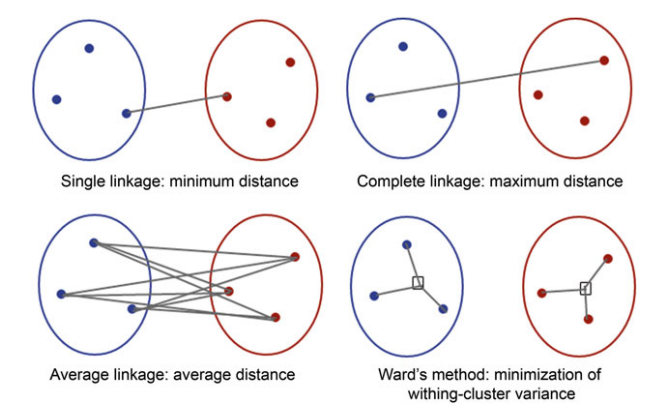
\includegraphics{./img/mod1/linkage_methods.png}\\
    \item
      \emph{Nearest neighbor (single linkage)}

      \begin{itemize}
      \tightlist
      \item
        Menor distância
      \end{itemize}
    \item
      \emph{Furthest neighbor (complete linkage)}

      \begin{itemize}
      \tightlist
      \item
        Maior distância
      \end{itemize}
    \item
      \emph{Between neighbor (average linkage)}

      \begin{itemize}
      \tightlist
      \item
        Distância média
      \end{itemize}
    \end{itemize}
  \end{itemize}
\item
  N Grupos

  \begin{itemize}
  \tightlist
  \item
    Critério

    \begin{itemize}
    \tightlist
    \item
      Pode-se adotar o tamanho do salto para a incorporação do seguinte

      \begin{itemize}
      \tightlist
      \item
        Saltos muito elevados indicam agrupamento de observações mais
        distintas\\
      \end{itemize}
    \item
      Comparar dendrogramas obtidos por diferentes métodos
    \end{itemize}
  \end{itemize}
\end{itemize}

\hypertarget{execuuxe7uxe3o}{%
\subsection{Execução}\label{execuuxe7uxe3o}}

\begin{itemize}
\tightlist
\item
  Objetivo

  \begin{itemize}
  \tightlist
  \item
    aglomerar iterativamente observações separadas em um único
    \emph{cluster}
  \end{itemize}
\item
  Algoritmo

  \begin{enumerate}
  \def\labelenumi{\arabic{enumi}.}
  \tightlist
  \item
    Inicia-se com n observações em n \emph{clusters}
  \item
    Une-se 2 observações com menos distância (sobram n-1
    \emph{clusters})
  \item
    Enquanto houver mais de 1 \emph{cluster}:

    \begin{itemize}
    \tightlist
    \item
      Um novo grupo é formado por:

      \begin{itemize}
      \tightlist
      \item
        união de 2 novas observações
      \item
        união de nova observação a um \emph{cluster}
      \end{itemize}
    \end{itemize}
  \item
    De posse do dengrograma, visualmente é possível definir o número de
    \emph{clusters} ao traçar uma linha horizontal no gráfico: o número
    de vezes que a linha corta o dendrograma indica quantos clusters
    formam-se naquele nível {[}{]}.
  \end{enumerate}
\item
  Visualização

  \begin{itemize}
  \tightlist
  \item
    dendrograma
  \end{itemize}
\item
  Dicas práticas

  \begin{itemize}
  \tightlist
  \item
    Dados que o objetivo é ter grupos mais homogêneos, deve-se evitar
    escolher o número de clusters em alturas muito altas, para que uma
    observação muito distinta faça parte do cluster.
  \item
    O melhor método de linkage em geral é feita visualmente mesmo,
    observando qual forma os melhores agrupamentos
  \item
    É possível observar o método de \emph{linkage} já ao gerar a matriz
    cofenética (de distâncias): se as distâncias forem muito pequenas e
    parecidas, provavelmente o \emph{complete linkage} terá mais
    sucesso. Se forem distantes, então talvez o \emph{single linkage}
    poderá resolver.
  \item
    Ao analisar um dendrograma resultante, ao traçarmos uma linha
    horizontal no gráfico, o número de vezes que a linha corta o
    dendrograma indica quantos clusters formam-se naquele nível.
  \end{itemize}
\end{itemize}

\hypertarget{anuxe1lise-dos-agrupamentos}{%
\subsection{Análise dos
agrupamentos}\label{anuxe1lise-dos-agrupamentos}}

\begin{itemize}
\tightlist
\item
  Quais variáveis contribuem?

  \begin{itemize}
  \tightlist
  \item
    O que

    \begin{itemize}
    \tightlist
    \item
      A variabilidade das variáveis métricas dentro do grupo é menor que
      do que a variabilidade entre grupos?
    \end{itemize}
  \item
    Como

    \begin{itemize}
    \tightlist
    \item
      Aplica-se teste F para análise de variância

      \begin{itemize}
      \tightlist
      \item
        \(F = \dfrac{\text{Variabilidade entre (extra) grupos}}{\text{Variabilidade dentro dos (intra) grupos}}\)
      \item
        Graus de liberdade no numerador: K-1
      \item
        Graus de liberdade no denominador: n-1
      \item
        K = nº clusters
      \item
        n = tamanho da amostra
      \end{itemize}
    \item
      Quanto maior o valor da estatística F, maior a relevância da
      variável para a formação de pelo menos um dos \emph{clusters}
    \end{itemize}
  \end{itemize}
\end{itemize}

\hypertarget{nuxe3o-hieruxe1rquico-k-means}{%
\section{Não Hierárquico K-Means}\label{nuxe3o-hieruxe1rquico-k-means}}

\hypertarget{tratamento-inicial-1}{%
\subsection{Tratamento inicial}\label{tratamento-inicial-1}}

\begin{itemize}
\tightlist
\item
  É sucetível a dados em escala diferentes

  \begin{itemize}
  \tightlist
  \item
    Necessário realizar padronização antes

    \begin{itemize}
    \tightlist
    \item
      \(ZX_{ji}=\dfrac{X_{ji}-\bar{X_j}}{S_j}\)
    \end{itemize}
  \end{itemize}
\end{itemize}

\hypertarget{escolhas-1}{%
\subsection{Escolhas}\label{escolhas-1}}

\begin{itemize}
\tightlist
\item
  Quantidade K de \emph{clusters} é escolhida a priori
\end{itemize}

\bookmarksetup{startatroot}

\hypertarget{introduction}{%
\chapter{Introduction}\label{introduction}}

This is a book created from markdown and executable code.

See Knuth (1984) for additional discussion of literate programming.

\bookmarksetup{startatroot}

\hypertarget{summary}{%
\chapter{Summary}\label{summary}}

In summary, this book has no content whatsoever.

\bookmarksetup{startatroot}

\hypertarget{references}{%
\chapter*{References}\label{references}}
\addcontentsline{toc}{chapter}{References}

\hypertarget{refs}{}
\begin{CSLReferences}{1}{0}
\leavevmode\vadjust pre{\hypertarget{ref-knuth84}{}}%
Knuth, Donald E. 1984. {``Literate Programming.''} \emph{Comput. J.} 27
(2): 97--111. \url{https://doi.org/10.1093/comjnl/27.2.97}.

\end{CSLReferences}



\end{document}
